%% -----------------------------------------------------------------
%% This file uses UTF-8 encoding
%%
%% For compilation use following command:
%% latexmk -pdf -pvc -bibtex --shell-escape thesis
%%
%% -----------------------------------------------------------------
%%                                     _     _      
%%      _ __  _ __ ___  __ _ _ __ ___ | |__ | | ___ 
%%     | '_ \| '__/ _ \/ _` | '_ ` _ \| '_ \| |/ _ \
%%     | |_) | | |  __/ (_| | | | | | | |_) | |  __/
%%     | .__/|_|  \___|\__,_|_| |_| |_|_.__/|_|\___|
%%     |_|                                          
%%
%% -----------------------------------------------------------------

\documentclass{kithesis}

% Additional packages
\usepackage[main=slovak,english]{babel}
\usepackage{blindtext}  % lorem ipsum
\usepackage{minted}  % for source code 

% Variables
%\thesisspec{figures/thesisspec.png} 

\title{My thesis \br (the skeleton)}{Moja záverečná práca \br (šablóna)}

\author{Janko Hraško}
\supervisor{Leslie Lamport} %veduci prace
\consultant{Donald E. Knuth} %konzultant
%\college{University of Žilina}{Žilinská univerzita} %univerzita
%\faculty{Faculty of Electrical Engineering and informatics}{Fakulta elektrotechniky a informatiky} %fakulta
%\department{Department of Computers and Informatics}{Katedra počítačov a informatiky} %katedra
%\departmentacr{DCI}{KPI} % skratka katedry
%\thesis{Master thesis}{Diplomová práca} %typ prace
\submissiondate{13}{5}{2016}
%\fieldofstudy{9.2.1 Informatika}
%\studyprogramme{Informatika}
%\city{Košice} %mesto
\keywords{\LaTeX, programming, typesetting}{\LaTeX, programovanie, sadzba textu}
%\declaration{som nepodvadzal}

\abstract{%
    % english 
	\blindtext
}{%
    % slovak 
	\blindtext
}

\acknowledgment{Na tomto mieste by som rád poďakoval svojmu vedúcemu práce za jeho čas a odborné vedenie počas riešenia mojej záverečnej práce.

Rovnako by som sa rád poďakoval svojim rodičom a priateľom za ich podporu a povzbudzovanie počas celého môjho štúdia.
    
V neposlednom rade by som sa rád poďakoval pánom \textit{Donaldovi E. Knuthovi} a \textit{Leslie Lamportovi} za typografický systém \LaTeX, s ktorým som strávil množstvo nezabudnuteľných večerov.}

\addbibresource{chapters/bibliography.bib}

% if you want to work only on selected chapters
%\includeonly{chapters/analyza} %,chapters/synteza}

% Load acronyms
% Acronyms
% ========
%
% An acronym is a word formed from the initial letters in a phrase. 
%
% Acronym Definition Exapmle:
% ---------------------------
% \newacronym{gcd}{GCD}{Greatest Common Divisor}
% \newacronym{dry}{DRY}{Don't Repeat Yourself}
%
% Usage:
% ------
% You can use these three options:
% 
% \acrlong{}  
%   Displays the phrase which the acronyms stands for. Put the label of the acronym inside the braces. In the example, \acrlong{gcd} prints Greatest Common Divisor. 
%
% \acrshort{} 
%   Prints the acronym whose label is passed as parameter. For instance, \acrshort{gcd} renders as GCD. 
%
% \acrfull{} 
%   Prints both, the acronym and its definition. In the example the output of \acrfull{dry} is Don't Repeat Yourself (DRY). 
% 
% For more information see:
% -------------------------
% * https://www.sharelatex.com/learn/Glossaries 
% * https://en.wikibooks.org/wiki/LaTeX/Glossary
%



%% -----------------------------------------------------------------
%%          _                                       _   
%%       __| | ___   ___ _   _ _ __ ___   ___ _ __ | |_ 
%%      / _` |/ _ \ / __| | | | '_ ` _ \ / _ \ '_ \| __|
%%     | (_| | (_) | (__| |_| | | | | | |  __/ | | | |_ 
%%      \__,_|\___/ \___|\__,_|_| |_| |_|\___|_| |_|\__|
%%                                                      
%% -----------------------------------------------------------------

\begin{document}
%% Title page, abstract, declaration etc.:
\frontmatter{}

%% List of code listings, if you are using package minted
%\listoflistings

%\pagenumbering{arabic}

%% Chapters
\chapter*{Motivácia}
\addcontentsline{toc}{chapter}{Motivácia}

\Blindtext

% !TEX root = ../thesis.tex

\chapter{Formulácia úlohy}

Text záverečnej práce musí obsahovať\/ kapitolu s~formuláciou úlohy resp. úloh riešených v~rámci záverečnej práce. V~tejto časti autor rozvedie spôsob, akým budú riešené úlohy a~tézy formulované v~zadaní práce. Taktiež uvedie prehľad podmienok riešenia.

\section{Anal\'yza}

Text záverečnej práce obsahuje kapitolu, v~rámci ktorej autor uvedie
analýzu riešených problémov. Táto kapitola môže byť v~prípade potreby
delená do viacerých podkapitol. Autor v~texte záverečnej práce môže
zvýrazniť kľúčové slová, pričom sa použije príslušný štýl pre kľúčové
slová -- napr. toto je kľúčové slovo. V~texte môžu byť použité obrázky
a~tabuľky podľa nasledujúcich príkladov:

\begin{figure}[!ht]
\centering \unitlength=1mm
\begin{picture}(30,30)(0,0)
\put(0,0){\line(1,0){30}}
\put(0,0){\line(0,1){30}}
\put(30,0){\line(0,1){30}}
\put(0,30){\line(1,0){30}}
\end{picture}
\caption{Toto je štvorec}\label{o:1}
\end{figure}


Obrázok by mal byť podľa možnosti centrovaný. Pri jeho opisovaní
v~texte treba použiť odkazy na obrázok v~tvare Obrázok~\ref{o:1}.

\tabcolsep=8pt
\begin{table}[!ht]\caption{Prehľad jednotiek}\label{t:1}
\smallskip
\centering
\begin{tabular}{|l|c|} \hline
Názov	& (Jednotka v~sústave SI) \\ \hline
Napätie & $\upmu$V \\ \hline
\end{tabular}
\end{table}
\nomenclature{$\upmu$}{mikro, $10^{-6}$}
\nomenclature{SI}{Syst\`eme International}
\nomenclature{V}{volt, základná jednotka napätia v sústave SI}

Tabuľka by mala byť podľa možnosti centrovaná. Pri jej opisovaní
v~texte treba použiť odkazy na tabuľku v~tvare: pozri
Tabuľku~\ref{t:1}. Na číslovanie obrázkov, resp. tabuliek treba použiť
triedenie. Za slovom {\it Obrázok} nasleduje ako prvé číslo kapitoly
alebo časti, v~ktorej sa obrázok nachádza, potom medzera, pomlčka,
medzera a~poradové číslo ilustrácie v~danej kapitole alebo časti.
Napr.:~Obrázok~\ref{o:1} (čiže: prvý obrázok v~druhej kapitole alebo
časti). V~prípade, ak tabuľka presahuje stranu, je možné použiť balík
\verb+longtable+.

Navrhujeme zaraďovať obrázky v~elektronickej podobe. Napríklad
Obrázok~\ref{o:2}, ktorý opisuje riešenie diferenciálnej rovnice
tlmených oscilácií
%% \def\ud{\mathrm{d}}
\begin{equation}\label{r:1}
\frac{\ud^2y}{\ud t^2}+\frac{\ud y}{\ud t}+y =0, \qquad y(0)=1, \quad
y\,'(0)=15,
\end{equation}
bol vytvorený v~MATLABe a~príkazom \texttt{print tlmosc.eps -f1
-deps2} bol uložený vo formáte Encapsulated Postscript. Na prípadné
použitie pdf\LaTeX{}u sa obrázok konvertuje do formátu PDF, napr.
pomocou programu \texttt{epstopdf}. Zvyčajne sa číslujú vzťahy, na
ktoré sa v~texte odvolávame. Napríklad: vzťahy (\ref{r:1}) definujú
Cauchyho začiatočnú úlohu.


\begin{figure}[ht!]
\centering
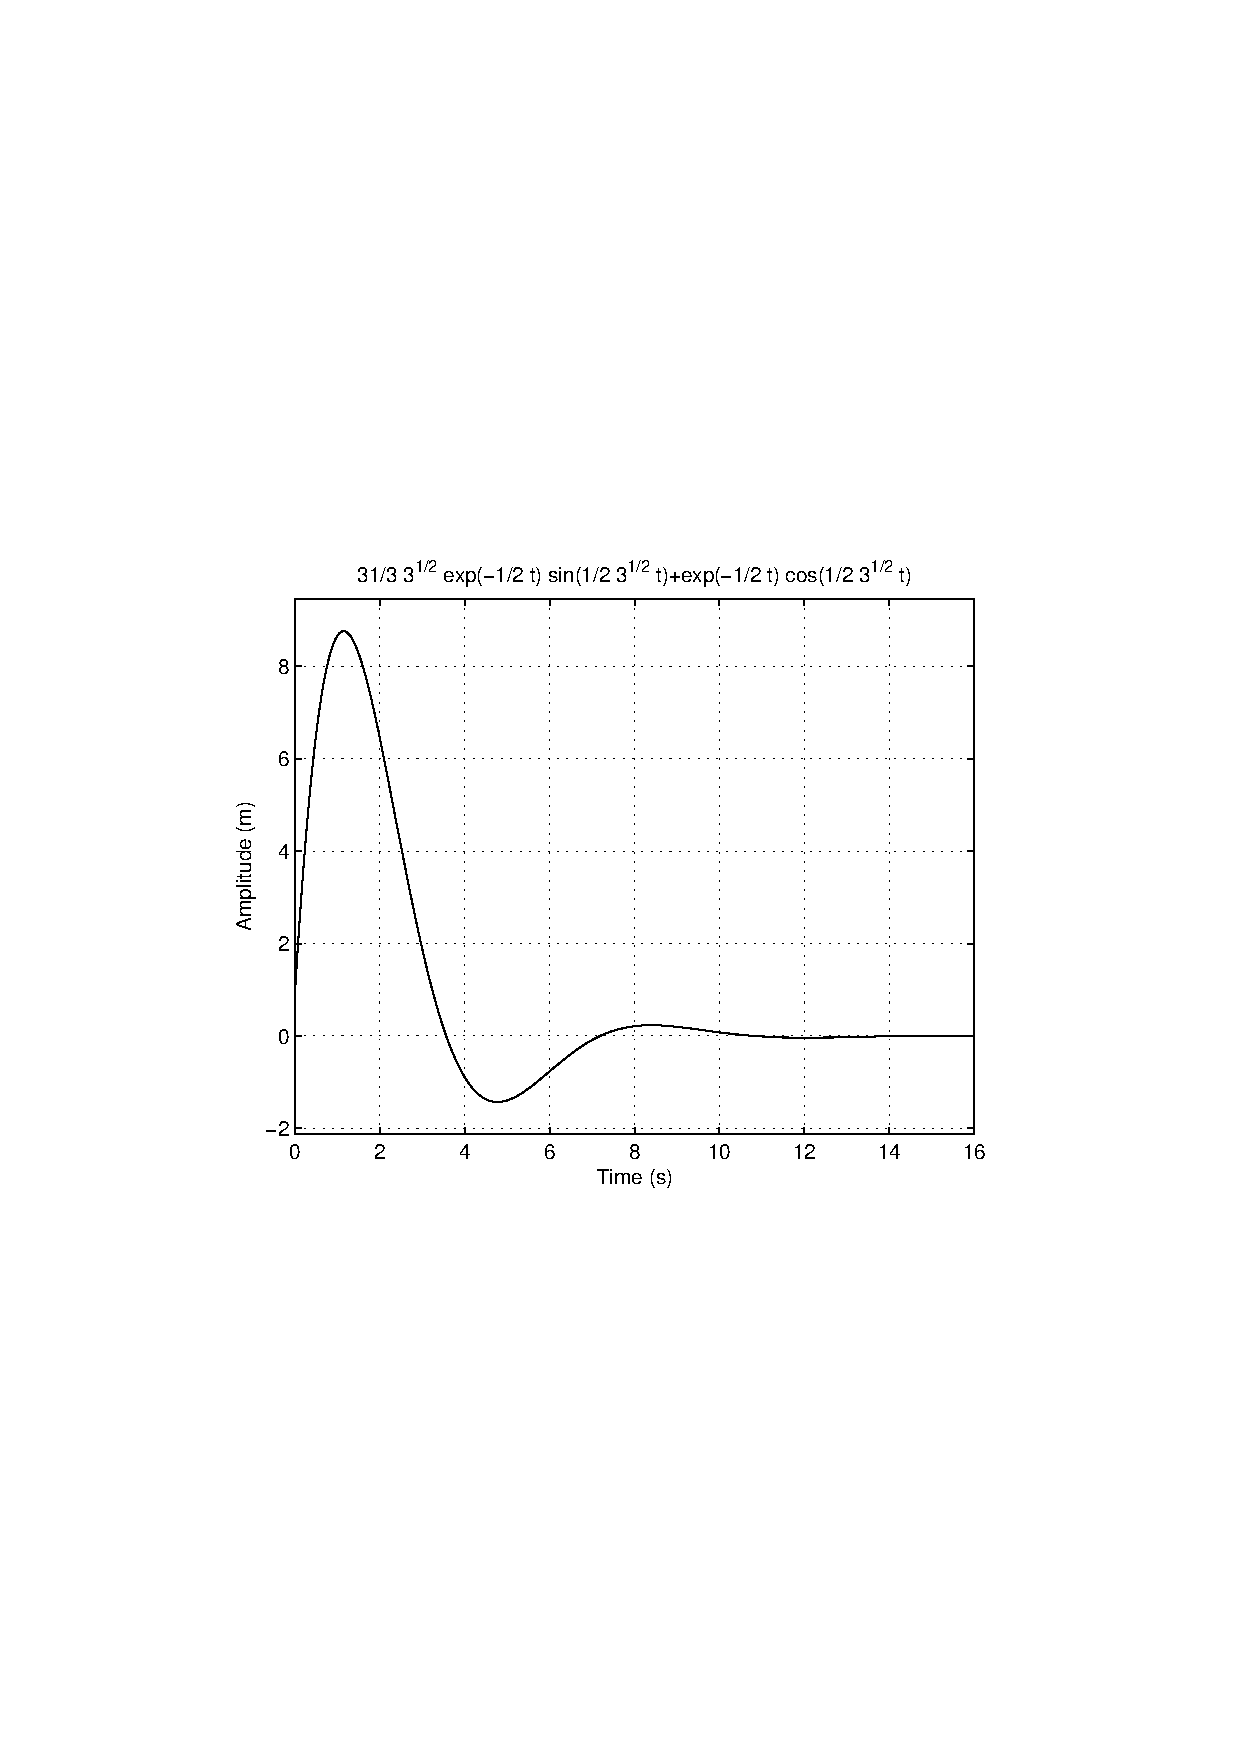
\includegraphics[width=0.7\textwidth]{tlmosc}
\caption{Grafické zobrazenie riešenia rovnice \ref{r:1}}\label{o:2}
\end{figure}



\subsection{Podkapitola}
Podkapitoly záverečnej práce majú za úlohu členenie textu záverečnej
práce s~cieľom, čo najväčšej prehľadnosti. Kapitol môže byť viacero
a~v~ich názvoch sa používa desatinné číslovanie.



\subsection{Vkladanie obrázkov}

Všetky obrázky, ktoré budete chcieť v dokumente použiť, ukladajte do priečinku {\tt figures/}. Následne obrázok vložte v prostredí \verb!figure! pomocou príkazu \verb!\includegraphics! bez uvedenia jeho prípony. Napríklad takto:

\begin{minted}{latex}
\begin{figure}[!ht]
	\centering
	
\includegraphics[width=\textwidth]{tugboat}
	\caption{\LaTeX{} priateľská zóna \label{o:latex\_friendly\_zone}}
\end{figure}

	\caption{Vloženie obrázku do textu dokumentu}
\end{minted}



\begin{figure}[!ht]
	\centering
	
\includegraphics[width=\textwidth]{tugboat}
	\caption{\LaTeX{} priateľská zóna \label{o:latex_friendly_zone}}
\end{figure}

% !TEX root = ../thesis.tex

\chapter{Syntetická časť práce}

% lorem ipsum
\blindtext
\blinditemize
\Blindtext
\Blindtext

% !TEX root = ../thesis.tex

\chapter{Vyhodnotenie}

% lorem ipsum
\blindtext
\blinditemize
\Blindtext
\Blindtext

% !TEX root = ../thesis.tex

\chapter{Záver}

% lorem ipsum
\Blindtext


% good linebraking of bibtex url
\setcounter{biburllcpenalty}{7000}
\setcounter{biburlucpenalty}{8000}

%% The bibliography
\printbibliography[heading=bibintoc,title={Literatúra}]

% List of acronyms
\printglossary[type=\acronymtype,title={\acrlistname}]

% Glossaries
\printglossary

%% Appendix
% !TEX root = ../thesis.tex

\chapter*{Zoznam príloh}
\addcontentsline{toc}{chapter}{Zoznam príloh}

\begin{description}
	\item[Príloha A] Karel Language Reference
    \item[Príloha B] CD médium -- záverečná práca v~elektronickej podobe,
    \item[Príloha C] Používateľská príručka
    \item[Príloha D] Systémová príručka
\end{description}

\appendix
\renewcommand\chaptername{Príloha}
% !TEX root = ../thesis.tex

\chapter{Systémová príručka}
Táto časť slúži na opis priečinkov a rozdelenia kódu.
\section*{Rozdelenie kódu}
Funkčný kód je rozdelený na dve časti. Prvá časť sa venuje základnej úprave dát do čitateľnej formy, konkrétne vo funkcii main napísanej v kóde java. Druhá časť, ktorá klasifikuje všetky dáta, spracováva výsledky a vypočítava skóre, je napísaná v Pythone, konkrétne v main funkcii predict.py. 
\section*{Opis kódu}
Prvá časť v kóde main.java má dve funkcie. Je to funkcia GetCharFromString, ktorá vracia aktuálny charakter v stringu a funkcia main, v ktorej otvoríme ako BufferedReader textový súbor 'menochampiona'+1.txt a zároveň vytvoríme nový textový súbor 'menochampiona'+.txt. Následne prechádzame celý textový súbor a upravujeme ho do čitateľnej podoby.
\\ Druhá čast v kóde predict.py má dve hlavné priority. Prvá je zápis všetkých získaných textových súborov z programu javy do jedného dataframu a zároveň ich klasifikácia. A druhá pracuje s daným dataframom a počíta skóre.
\section*{Opis priečinkov}
V priečinku transformdata sa nachádza 332 súborov, z čoho je viac než 320 textových súborov s dátami o každom jednom šampiónovi. Zároveň je tam aj hlavná časť kódu a to súbor predict.py, ktorý má v sebe spracovanie a úpravu všetkých dát. Hlavný súbor s dátami sa volá winratedata.txt ktorý v sebe drží hodnoty všetkých klasifikovaných dát pre každého šampióna. Takisto v hlavnom priečinku môžete nájsť vysledky.xlsx, čo je excelovská tabuľka všetkých otestovaných zápasov. V priečinku src nájdeme kód main.java, pomocou ktorého sme dáta dostali do čitateľnej podoby pre náš python kód. 

\chapter{Používateľská príručka}
V tejto časti si ukážeme ako spustiť a obsluhovať aktuálny kód.

\section*{Potrebné súbory}
Na úspešné odskúšanie kódu na predikciu potrebujete mať textové súbory winratedata.txt, winlose.txt, teams.txt a zároveň samotný súbor s kódom predict.py, ktorý sa nachádza v hlavnom priečinku spolu s textovými súbormi.

\section*{Príprava prostredia a knižníc} 
Odporúčané prostredie je Spyder, ideálne verzia 5.0.5 a novšie. Prostredie Spyder je možné stiahnuť na ich domácej stránke zadarmo. Potrebná knižnica na stiahnutie je pandas, čo môžete vykonať príkazom - pip install pandas, napísaným v konzole.

\section*{Popis používania}
Kód predict.py je potrebné otvoriť v predpripravenom prostredí. Následne na vrchu kódu je 5 premenných top, jg, mid, bot a sup. Pri predikcii kompozície, ktorú chcete odskúšať do týchto premenných, vložte mená šampiónov bez medzier v ich mene s malými písmenami. Ak ste tak vykonali, spustite kód zelenou šípkou a v konzole by mali byť vypísané premenné totalgames, totalscore a známka, čo označuje aktuálnu kompozíciu, ktorú ste zapísali. 


% zivotopis autora
%\curriculumvitae\protect
%Táto časť\/ je nepovinná. Autor tu môže uviesť\/ svoje biografické
%údaje, údaje o~záujmoch, účasti na~projektoch, účasti na~súťažiach,
%získané ocenenia, zahraničné pobyty na~praxi, domácu prax, publikácie
%a~pod.

\end{document}
